\begin{figure}[h!]
	\centering
	
	
	\tikzset{every picture/.style={line width=0.75pt}} %set default line width to 0.75pt        
	
	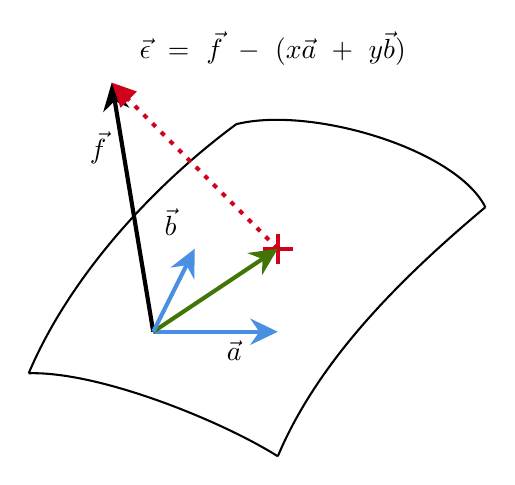
\begin{tikzpicture}[x=0.75pt,y=0.75pt,yscale=-1,xscale=1]
		%uncomment if require: \path (0,300); %set diagram left start at 0, and has height of 300
		
		%Curve Lines [id:da8629621226111777] 
		\draw    (200,220) .. controls (234,219) and (293,243) .. (320,260) ;
		%Curve Lines [id:da7503332355924262] 
		\draw    (200,220) .. controls (219,175) and (258,131) .. (300,100) ;
		%Curve Lines [id:da4421062117367349] 
		\draw    (320,260) .. controls (339,215) and (377,176) .. (420,140) ;
		%Curve Lines [id:da09638310751018486] 
		\draw    (300,100) .. controls (336,91) and (406,112) .. (420,140) ;
		%Straight Lines [id:da011060636069030183] 
		\draw [color={rgb, 255:red, 74; green, 144; blue, 226 }  ,draw opacity=1 ][line width=1.5]    (260,200) -- (316,200) ;
		\draw [shift={(320,200)}, rotate = 180] [fill={rgb, 255:red, 74; green, 144; blue, 226 }  ,fill opacity=1 ][line width=0.08]  [draw opacity=0] (13.4,-6.43) -- (0,0) -- (13.4,6.44) -- (8.9,0) -- cycle    ;
		%Straight Lines [id:da4073170813949978] 
		\draw [line width=1.5]    (260,200) -- (240.66,83.95) ;
		\draw [shift={(240,80)}, rotate = 80.54] [fill={rgb, 255:red, 0; green, 0; blue, 0 }  ][line width=0.08]  [draw opacity=0] (13.4,-6.43) -- (0,0) -- (13.4,6.44) -- (8.9,0) -- cycle    ;
		%Straight Lines [id:da2813040556316886] 
		\draw [color={rgb, 255:red, 208; green, 2; blue, 27 }  ,draw opacity=1 ][line width=1.5]  [dash pattern={on 1.69pt off 2.76pt}]  (242.83,82.83) -- (320,160) ;
		\draw [shift={(320,160)}, rotate = 90] [color={rgb, 255:red, 208; green, 2; blue, 27 }  ,draw opacity=1 ][line width=1.5]    (-7.27,0) -- (7.27,0)(0,7.27) -- (0,-7.27)   ;
		\draw [shift={(240,80)}, rotate = 45] [fill={rgb, 255:red, 208; green, 2; blue, 27 }  ,fill opacity=1 ][line width=0.08]  [draw opacity=0] (11.61,-5.58) -- (0,0) -- (11.61,5.58) -- cycle    ;
		%Straight Lines [id:da36335814673507816] 
		\draw [color={rgb, 255:red, 65; green, 117; blue, 5 }  ,draw opacity=1 ][line width=1.5]    (260,200) -- (316.67,162.22) ;
		\draw [shift={(320,160)}, rotate = 146.31] [fill={rgb, 255:red, 65; green, 117; blue, 5 }  ,fill opacity=1 ][line width=0.08]  [draw opacity=0] (13.4,-6.43) -- (0,0) -- (13.4,6.44) -- (8.9,0) -- cycle    ;
		%Straight Lines [id:da9021313863216152] 
		\draw [color={rgb, 255:red, 74; green, 144; blue, 226 }  ,draw opacity=1 ][line width=1.5]    (260,200) -- (278.21,163.58) ;
		\draw [shift={(280,160)}, rotate = 116.57] [fill={rgb, 255:red, 74; green, 144; blue, 226 }  ,fill opacity=1 ][line width=0.08]  [draw opacity=0] (13.4,-6.43) -- (0,0) -- (13.4,6.44) -- (8.9,0) -- cycle    ;
		
		% Text Node
		\draw (294,203) node [anchor=north west][inner sep=0.75pt]   [align=left] {$\displaystyle \vec{a}$};
		% Text Node
		\draw (264,139) node [anchor=north west][inner sep=0.75pt]   [align=left] {$\displaystyle \vec{b}$};
		% Text Node
		\draw (252,54) node [anchor=north west][inner sep=0.75pt]   [align=left] {$\displaystyle \vec{\epsilon } \ =\ \vec{f} \ -\ ( x\vec{a} \ +\ y\vec{b})$};
		% Text Node
		\draw (228,102) node [anchor=north west][inner sep=0.75pt]   [align=left] {$\displaystyle \vec{f}$};
		
		
	\end{tikzpicture}
	\caption{Geometrical interpretation of a 3 dimensional over determined system of equations.}
\end{figure}